% -*- latex -*-
%%%%%%%%%%%%%%%%%%%%%%%%%%%%%%%%%%%%%%%%%%%%%%%%%%%%%%%%%%%%%%%%
%%%%
%%%% This TeX file is part of the course
%%%% Introduction to Scientific Programming in C++/Fortran2003
%%%% copyright 2017-2023 Victor Eijkhout eijkhout@tacc.utexas.edu
%%%%
%%%% tdd.tex : unit testing and test-driven development
%%%%
%%%%%%%%%%%%%%%%%%%%%%%%%%%%%%%%%%%%%%%%%%%%%%%%%%%%%%%%%%%%%%%%

In an ideal world, you would prove your program correct,
but in practice that is not always feasible,
or at least: not done.
Most of the time programmers establish the correctness of their code
by testing it.

Yes, there is a quote by \indextermsub{Edsger}{Dijkstra} that goes:
\begin{quotation}
  Today a usual technique is to make a program and then to test
  it. But: program testing can be a very effective way to show the
  presence of bugs, but is hopelessly inadequate for showing their
  absence. (cue laughter)
\end{quotation}
but that doesn't mean that you can't at least gain some confidence
in your code by testing it.

\Level 0 {Types of tests}

Testing code is an art, even more than writing the code to begin with.
That doesn't mean you can't be systematic about it.
First of all, we distinguish between some basic types of test:
\begin{itemize}
\item \emph{Unit tests}\index{unit test|see{testing, unit}}\index{testing!unit}
  that test a small part of a program by itself;
\item \emph{System tests}\index{system test!see{testing, system}}\index{testing!system}
  test the correct behavior of the whole software system; and
\item \emph{Regression tests}\index{regression test!see{testing, regression}}\index{testing!regression}
  establish that the behavior of a program has not changed by adding or changing aspects of it.
\end{itemize}
In this section we will talk about unit testing.

A program that is written in a sufficiently  modular way
allows for its components to be tested
without having to wait for an all-or-nothing test of the whole program.
Thus, testing and program design are aligned in their interests.
In fact, writing a program with the thought in mind that it needs to be testable
can lead to cleaner, more modular code.

In an extreme form of this you would write
your code by \acf{TDD}, where code development and testing
go hand-in-hand. The basic principles can be stated as follows:
\begin{itemize}
\item Both the whole code and its parts should always be testable.
\item When extending the code, make only the smallest change that allows for testing.
\item With every change, test before and after.
\item Assure correctness before adding new features.  
\end{itemize}
In a strict interpretation,
you would even for each part of the
program first write the test that it would satisfy,
and then the actual code.

\Level 0 {Unit testing frameworks}
\label{sec:tdd}

There are several `frameworks' that help you with unit testing.
In the remainder of this chapter we will use \indexterm{Catch2},
which is one of the most used ones in~C++.

You can find the code at \url{https://github.com/catchorg}.

\begin{figure}[t]
  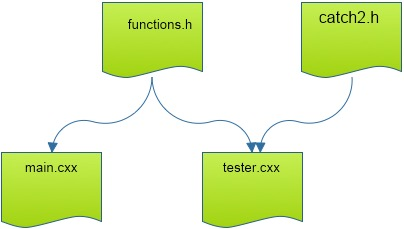
\includegraphics{catch2main}
  \caption{File structure for unit tests}
  \label{fig:catch2main}
\end{figure}

\Level 1 {File structure}

Let's assume you have a file structure with
\begin{itemize}
\item a very short main program, and
\item a library file that has all functions used by the main.
\end{itemize}
In order to test the functions, you supply another main,
which contains only unit tests;  
This is illustrated in figure~\ref{fig:catch2main}.

In fact, with Catch2 your main file doesn't actually have
a \lstinline{main} program: that is supplied by the framework.
In the tester main file you only put the test cases.

\begin{block}{Unittest driver file}
  \label{sl:catch2main}
The framework supplies its own main:
\begin{lstlisting}
#define CATCH_CONFIG_MAIN
#include "catch2/catch_all.hpp"

#include "library_functions.h"
/*
   here follow the unit tests
*/
\end{lstlisting}
\end{block}

One important question is what header file to include.
You can do 
\begin{lstlisting}
#include "catch.hpp"
\end{lstlisting}
which is the `header only' mode,
but that makes compilation very slow.
Therefore, we will assume you have installed Catch through \indexterm{Cmake},
and you include
\begin{lstlisting}
#include "catch2/catch_all.hpp"
\end{lstlisting}
Note: as of September 2021 this requires the development version of the repository,
not any \n{2.x} release.

\Level 1 {Compilation}

The setup suggested above requires you to add compile and link flags to your setup.
This is system-dependent.

\begin{tacc}
\begin{block}{Compiling the tester at TACC}
\label{sl:catch-compile}
One-line solution:
\begin{verbatim}
icpc -o tester test_main.cxx \
    -I${TACC_CATCH2_INC} -L${TACC_CATCH2_LIB} \
    -lCatch2Main -lCatch2
\end{verbatim}
\end{block}
\begin{block}{Compile and link options at TACC}
\label{sl:catch-compile-options}
Variables for a Makefile:
\begin{verbatim}
INCLUDES = -I${TACC_CATCH2_INC}
EXTRALIBS = -L${TACC_CATCH2_LIB} -lCatch2Main -lCatch2
\end{verbatim}
\end{block}
\end{tacc}

\Level 1 {Test cases}

A test case is a short program that is run as an independent main.
In the setup suggested above, you put all your unit tests
in the tester main program, that is,
the file that has the
\begin{lstlisting}
#define CATCH_CONFIG_MAIN
#include "catch2/catch_all.hpp"
\end{lstlisting}
magic lines.

Each test case needs to have a unique name,
which is printed when a test fails.
You can optionally add keys to the test case
that allow you to select tests from the commandline.

\begin{lstlisting}
TEST_CASE( "name of this test" ) {
  // stuf
}
TEST_CASE( "name of this test","[key1][key2]" ) {
  // stuf
}
\end{lstlisting}

The body of the test case is essentially a main program,
where some statements are encapsulated in test macros.
The most common macro is \lstinline{REQUIRE},
which is used to demand correctness of some condition.

\begin{block}{Correctness through `require' clause}
  \label{sl:catch-case-require}
Tests go in \n{tester.cxx}:
\begin{lstlisting}
TEST_CASE( "test that f always returns positive" ) {
  for (int n=0; n<1000; n++)
    REQUIRE( f(n)>0 );  
}
\end{lstlisting}
\begin{itemize}
  \item
    \lstinline+TEST_CASE+ acts like independent main program.\\
    can have multiple cases in a tester file
    \item \lstinline{REQUIRE} is like \n{assert} but more sophisticated
  \end{itemize}
\end{block}

\begin{exercise}
  \label{ex:catch-example}
  \begin{enumerate}
  \item Write a function
\begin{lstlisting}
double f(int n) { /* .... */ }
\end{lstlisting}
    that takes on positive values only.
  \item Write a unit test that tests the function for a number of values.
  \end{enumerate}
  \skeleton{tdd}
\end{exercise}

\begin{block}{Tests}
  \label{sl:catch-approx}
  Boolean:
\begin{lstlisting}
REQUIRE( some_test(some_input) );
REQUIRE( not some_test(other_input) );
\end{lstlisting}
Integer:
\begin{lstlisting}
REQUIRE( integer_function(1)==3 );
REQUIRE( integer_function(1)!=0 );
\end{lstlisting}
Beware floating point:
\begin{lstlisting}
REQUIRE( real_function(1.5)==Catch::Approx(3.0) );
REQUIRE( real_function(1)!=Catch::Approx(1.0) );
\end{lstlisting}
In general exact tests don't work.
\end{block}

For failing tests, the framework will give
the name of the test, the line number,
and the values that were tested.

\begin{block}{Output for failing tests}
  \label{sl:catch-fail}
  \small
  Run the tester:
\begin{verbatim}
--------------------------------
test the increment function
--------------------------------
test.cxx:25
................................

test.cxx:29: FAILED:
  REQUIRE( increment_positive_only(i)==i+1 )
with expansion:
  1 == 2

================================
test cases: 1 | 1 failed
assertions: 1 | 1 failed
\end{verbatim}
\end{block}

In the above case, the error message
printed out the offending value of \lstinline+f(n)+,
not the value of \lstinline+n+ for which it occurs.
To determine this, insert \lstinline+INFO+ specifications,
which only get print out if a test fails.

\begin{block}{Diagnostic information for failing tests}
  \label{sl:catch-info}
  \n{INFO}: print out information at a failing test
\begin{lstlisting}
TEST_CASE( "test that f always returns positive" ) {
  for (int n=0; n<1000; n++)
    INFO( "function fails for " << n );
    REQUIRE( f(n)>0 );  
}  
\end{lstlisting}
\end{block}

If your code throws exceptions (section~\ref{sec:exception})
you can test for these.

\begin{block}{Test for exceptions}
  \label{sl:catch-case-throw}
Suppose function \n{g(n)}
\begin{itemize}
\item succeeds for input $n>0$
\item fails for input $n\leq 0$:\\ throws exception
\end{itemize}

\begin{lstlisting}
TEST_CASE( "test that g only works for positive" ) {
  for (int n=-100; n<+100; n++)
    if (n<=0)
      REQUIRE_THROWS( g(n) );  
    else
      REQUIRE_NOTHROW( g(n) );  
}
\end{lstlisting}
\end{block}

A common occurrence in unit testing is to have
multiple tests with a common setup or tear down,
to use terms that you sometimes come across in unit testing.
Catch2 supports this:
you can make `sections' for part in between setup and tear down.

\begin{block}{Tests with code in common}
\label{sl:catch-section}
Use \n{SECTION} if tests have intro/outtro in common:
\begin{lstlisting}
TEST_CASE( "commonalities" ) {
  // common setup:
  double x,y,z;
  REQUIRE_NOTHROW( y = f(x) );
  // two independent tests:
  SECTION( "g function" ) {
    REQUIRE_NOTHROW( z = g(y) );
  }
  SECTION( "h function" ) {
    REQUIRE_NOTHROW( z = h(y) );
  }
  // common followup
  REQUIRE( z>x );
}
\end{lstlisting}
(sometimes called setup/teardown)
\end{block}

\Level 0 {Example: zero-finding by bisection}

Development of the zero-finding algorithm by bisection
can be found in section~\ref{sec:root-bisection}.

\Level 0 {An example: quadratic equation roots}
\label{sec:quad-tdd}

We revisit exercise~\ref{ex:quad-roots},
which used \indexcstd{variant}
to return 0,1,2 roots of a quadratic equation.
Here we use \ac{TDD} to arrive at the code.

Throughout, we represent the polynomial
\[ ax^2+bx+c \]
as 
\begin{lstlisting}
using quadratic = tuple<double,double,double>;  
\end{lstlisting}
When needed, you can unpack this again with
\begin{lstlisting}
auto [a,b,c] = coefficients;  
\end{lstlisting}
(Can you think of an \indexc{assert} statement here
that might be useful?)

\begin{exercise}
  \label{ex:qdisc}
  Write a function
\begin{lstlisting}
double discriminant( quadratic coefficients );
\end{lstlisting}
that computes $b^2-4ac$, and test:
\codesnippet{qtestdiscriminant}
\end{exercise}

It may be illustrative to see what happens if you leave out the
approximate equality test:
\begin{lstlisting}
REQUIRE( discriminant( make_tuple(.1, .1, .1*.5 ) ) == -.01 );
\end{lstlisting}

With this function it becomes easy to detect the case of no roots:
the discriminant~$D<0$.
Next we need to have the criterium for single or double roots:
we have a single root if~$D=0$.

\begin{exercise}
  \label{ex:qdisczero}
  Write a function
\begin{lstlisting}
bool discriminant_zero( quadratic coefficients );
\end{lstlisting}
that passes the test
\codesnippet{qtestdzero}
Using for instance the values:
\begin{lstlisting}
a = 2; b = 4; c = 2;
a = 2; b = sqrt(40); c = 5; // !!!
a = 3; b = 0; c = 0.;
\end{lstlisting}
\end{exercise}

This exercise is the first one where we run into
numerical subtleties.
The second set of test values has the discriminant zero
in exact arithmetic, but nonzero in computer arithmetic.
Therefore, we need to test whether it is small enough, compared to~$b$.

\begin{exercise}
  Be sure to also test the case where \lstinline+discriminant_zero+
  returns false.
\end{exercise}

Now that we've detected a single root, we need the function
that computes it. There are no subtleties in this one.

\begin{exercise}
  \label{ex:qtestsimple}
  Write the function \lstinline+simple_root+ that returns
  the single root.
  For confirmation, test
  \codesnippet{qtestsimple}
\end{exercise}

The remaining case of two distinct roots is arrived at
by elimination, and the only thing to do is write
the function that returns them.

\begin{exercise}
  \label{ex:qtestdouble}
  Write a function that returns the two roots
  as a \\indexcstd{pair}:
\begin{lstlisting}
pair<double,double> double_root( quadratic coefficients );
\end{lstlisting}
Test:
\codesnippet{qtestdouble}
\end{exercise}

The final bit of code is the function that
tests for how many roots there are, and returns them
as a \indexcstd{variant}.

\begin{exercise}
  \label{ex:qtestfull}
  Write a function
\begin{lstlisting}
variant< bool,double, pair<double,double> > 
    compute_roots( quadratic coefficients);
\end{lstlisting}
Test:
\begin{multicols}{2}
  \codesnippet{qtestfull}
\end{multicols}
\end{exercise}

\Level 0 {Eight queens example}

See \ref{sec:8queens-tdd}.
